\chapter{内存管理}
在计算机系统(1)中,我们在虚拟存储器部分引出了交换空间的概念。管理内存是硬件和软件协同的结果。
在CPU启动后,内存的地址空间完整提供给第一个启动的软件,也就是操作系统。
随后操作系统在创建每一个进程时分配页表进行页映射,从而提供每个进程完整虚拟地址空间的抽象。
在这个专题的实践中,我们的目标是体验操作系统中不同的内存类型和对应管理内存的方式。

\section{页表和文件页}
目标:读取页表,并且手动修改页表页的映射实现共享(通过\texttt{mmap}调整映射,通过修改内核读取页表);设置文件页实现读写落在文件的指定区域中。

测试:测试页表映射和修改是否生效到文件中。

\section{内存文件系统}
Linux中提供了内存文件系统(RAMfs)的支持,其有MMU版本和NoMMU版本,分别位于\texttt{fs/ramfs/file-mmu.c}和\texttt{fs/ramfs/file-nommu.c}。
RAMfs无法持久化,在系统崩溃时文件会全部丢失。
现在你需要为RAMfs提供简单的持久化支持,当某个文件被flush到RAMfs时,该文件同步刷到一个预先设置的同步目录中以持久化该文件。

目标:增加flush下的文件持久化。

测试:测试持久化的文件内容语义和多线程持久化。



\section{内存压力导向的内存管理}
MacOS给出内存压力的概念,相比于UNIX的swap大小,它被认为是更好的表达虚拟内存健康程度的标志。

\begin{figure}[h]
    \centering
    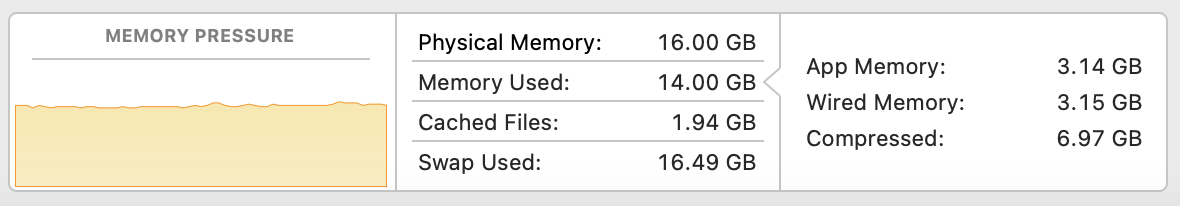
\includegraphics[width=0.8\linewidth]{figure/mixed-figures/memory-pressure.png}
    \caption{MacOS中的内存压力}
    \label{fig:enter-label}
\end{figure}

目标:该实践任务包含两个子任务点。
\begin{enumerate}
    \item 利用Linux的Wired Memory(即Active Memory)和压缩内存给出一个Linux下的内核内存压力指示器。
    \item 在用户态划出一块内存空间,实现一个简单的基于内存压力的交换策略。
\end{enumerate}


提示:区分wired memory和inactive memory的区别。

测试:测试内存压力和感知准确度的对比(演示),测试交换策略。
